% Template for Cogsci submission with R Markdown

% Stuff changed from original Markdown PLOS Template
\documentclass[10pt, letterpaper]{article}

\usepackage{cogsci}
\usepackage{pslatex}
\usepackage{float}
\usepackage{caption}

% amsmath package, useful for mathematical formulas
\usepackage{amsmath}

% amssymb package, useful for mathematical symbols
\usepackage{amssymb}

% hyperref package, useful for hyperlinks
\usepackage{hyperref}

% graphicx package, useful for including eps and pdf graphics
% include graphics with the command \includegraphics
\usepackage{graphicx}

% Sweave(-like)
\usepackage{fancyvrb}
\DefineVerbatimEnvironment{Sinput}{Verbatim}{fontshape=sl}
\DefineVerbatimEnvironment{Soutput}{Verbatim}{}
\DefineVerbatimEnvironment{Scode}{Verbatim}{fontshape=sl}
\newenvironment{Schunk}{}{}
\DefineVerbatimEnvironment{Code}{Verbatim}{}
\DefineVerbatimEnvironment{CodeInput}{Verbatim}{fontshape=sl}
\DefineVerbatimEnvironment{CodeOutput}{Verbatim}{}
\newenvironment{CodeChunk}{}{}

% cite package, to clean up citations in the main text. Do not remove.
\usepackage{apacite}

% KM added 1/4/18 to allow control of blind submission
\cogscifinalcopy

\usepackage{color}

% Use doublespacing - comment out for single spacing
%\usepackage{setspace}
%\doublespacing


% % Text layout
% \topmargin 0.0cm
% \oddsidemargin 0.5cm
% \evensidemargin 0.5cm
% \textwidth 16cm
% \textheight 21cm

\title{Understanding the impact of electronically-delivered parenting advice}


\author{{\large\bf Hanwen Vivian~Zhang} (\texttt{vivian3@stanford.edu}) \\ {\large\bf George~Kachergis} (\texttt{george.kachergis@gmail.com}) \\ {\large\bf Michael C.~Frank} (\texttt{mcfrank@stanford.edu}) \\  Department of Psychology, Stanford University \\  Stanford, CA 94305 USA}

\begin{document}

\maketitle

\begin{abstract}
Early parenting practices play an important role in shaping the future
outcomes of young children (Hart \& Risley, 1995; Heckman, 2006). In
particular, high-quality early interactions and language input appear to
facilitate language learning and result in higher levels of school
performance. The rise of phone- and tablet-based parenting applications
(``apps'') holds the promise of delivering low-cost, positive
interventions on parenting style to a variety of different populations.
Of special interest are the parents of very young children, who are
often difficult to reach in other ways. Yet little is known about the
effects of communicating to parents through app-based interventions. In
a study of one commercial app offering a collection of age-appropriate
activity videos, we find that the quality of parent-child interactions
increases in some ways as a result of using the app. Specifically, the
lexical diversity of parents' child-directed speech increases, and
measures of joint attention show\ldots{}

\textbf{Keywords:}
digital parenting advice; joint attention; lexical diversity; guided
play;
\end{abstract}

\section{Introduction}\label{introduction}

Young children spend a large portion of their waking time at play,
variously manipulating objects, exploring their environment, and
interacting with caregivers and peers. Playing with objects allows them
to discover hidden object properties and relations, and to build a
causal understanding of how objects interact (e.g., Schulz \& Bonawitz,
2007). Meanwhile, play also gives children an opportunity to set and
achieve goals (e.g., build a tower) and to practice a wide range of
motor skills (e.g., stacking) that will help them navigate the world
(Singer, Golinkoff, \& Hirsh-Pasek, 2006). Social play can help children
learn about human relationships, both through imitation of adult
behaviors and by experiencing and learning to process emotional events
such as failures (Singer et al., 2006). Of course, young children are
rarely playing in isolation: caregivers often provide encouragement and
guidance while scaffolding a child's play (Kaye, 1970; Wood, Bruner, \&
Ross, 1976). Indeed, parenting practices early in childhood have been
shown to play an important role in shaping the future outcomes of young
children (Hart \& Risley, 1995; Heckman, 2006). While interventions
often have trouble reaching many parents of very young children, the
proliferation of mobile devices offers a good avenut for the digital
delivery of parenting advice (Breitenstein, Gross, \& Christophersen,
2014).

\subsection{Guided Play Scaffolds
Learning}\label{guided-play-scaffolds-learning}

Children's early play behaviors are often assisted by more skilled and
knowledgeable play partners such as their caregivers and older siblings
(Kaye, 1970). Under such expert guidance, children are encouraged and
motivated to engage in more advanced play, undertaking explorations that
push the boundaries of what they would be able to do unaided (Vygotsky,
1980). These tutorial interactions have been shown to be important
components of child development (Wood et al., 1976). Thus, with the
knowledge of both play and tutorial interactions, guided play, which
consists of both active and enjoyable activities as well as close
guidance of adults (Hirsh-Pasek \& Golinkoff, 2008) has drawn
researchers' interest. A study of preschoolers showed that guided play
scaffolds the environment while still allowing children to maintain a
large degree of control, and it outperforms direct-instruction
approaches in encouraging a variety of positive academic outcomes
(Weisberg, Hirsh-Pasek, \& Golinkoff, 2013). Another study found that
guided play could facilitate children's vocabulary and comprehensive
language development and subsequent literacy skills (Massey, 2013).

\subsection{Improving Parenting Practices and Language
Use}\label{improving-parenting-practices-and-language-use}

Thus, including guided play in parenting practices early on is crucial
and will help with children's later performances in academic and social
situations. To intervene in parenting practices, Suskind and others did
a parent-directed home-visiting intervention experiment in 2015 for
children of low socioeconomic status. They showed that parents in
experimental group have greater knowledge of language development and
this effect sustained four months after the intervention. However,
although a number of interactive measures increased during the
experiment, including the number of word tokens, conversational turns,
and child vocalizations, these increases did not sustain after the
intervention (D. L. Suskind et al., 2015). That changes did not sustain
could be due to the intervention itself, or could merely be that the
methods of home-visiting is not sustainable enough for parents to easily
and constantly get parenting advice. Thus, new methods of delivering
parenting advice should be considered.

\subsection{Effectiveness of Digital
Delivery}\label{effectiveness-of-digital-delivery}

With the widespread use of smartphones and tablets worldwide,
digitally-delivered interventions could address many of the logistical
barriers that have limited scaling up face-to-face delivery methods. A
review of 11 studies verified that digital delivery is a promising means
of effectively distributing interventions (Breitenstein et al., 2014).
However, the parent and child outcomes assessed in the review
(e.g.infant positive behaviors, satisfaction, emotional symptoms etc.)
did not address the nature or quality of parent-infant interactions at a
detailed level, like if the interventions lead to children paying more
attention, or vocabulary changes in parents' language usages. Although
digitally-delivered ac-tivities are designed to promote learning and
cognitive development, it is unclear how they might affect these
dimensions of parent-child interactions. Thus, we want to conduct this
experiment to explore if and how digital scaffolding of activities
affect the social and linguistic characteristics of parent-child
ineractions. The quality of parent-child interactions can be measured by
both the social engagement of parents (e.g., joint attention to objects
in the environment)(Bigelow, MacLean, \& Proctor, 2004) and the quality
of language (e.g., vocabulary diversity) (Malvern, Richards, Chipere, \&
Durán, 2004).

\section{Experiment 1}\label{experiment-1}

In Experiment 1, we invited parents of 6- to 24-month-old infants
visiting the Children's Discovery Museum in San Jose to complete
activities from the Kinedu app. Parents were randomly assigned to the
video group or the control group; parents in the video group watched a
video from the Kinedu app (matched to their child's age), and then
performed the activity with their child using the props from the video.
Parents in the control group did not watch a Kinedu video, instead they
were given the same props and were told to play with their infants as
they would at home.

\subsection{Method}\label{method}

\subsubsection{Participants.}\label{participants.}

60 infants (F = 42, M = 18) aged 6-24 months (20 6-11.9 month-olds, 20
12-17.9 month-olds, and 20 18-24 month-olds) and their parents
participated in a museum in northern California. We included infants who
were exposed to English at least 50 percent of the time (n = 58) or who
were exposed less but whose participating parent reported that they
primarily speak English with their child at home (n = 2). Sixty-one\% of
participants (n = 37) had been exposed to two or more languages as
indicated by their parent. Parents identified their children as White (n
= 25), Asian (n = 11), African American/Black (n = 2), Biracial (n =
12), other (n = 5), or declined to state (n = 5). Fifteen parents
reported their child was of Hispanic origin. Parents tended to be
highly-educated, with reports of highest level of education ranging from
completed high school (n = 5), some college (n = 6), four-year college
(n = 14), some graduate school (n = 1), to completed graduate school (n
= 28) or declined to state (n = 6).

\subsubsection{Materials.}\label{materials.}

Stimuli included videos from the Kinedu (Kinedu Inc.) commercial
parenting application. The videos were designed to show activities to
parents that they could perform with their child in order to foster
cognitive and physical development, and were targeted to the child's age
and level of development. In each video, an adult and child perform the
activity while a narrator explains the activity and its purpose. We
selected two videos for each of three age groups in our sample (6-11.9
months, 12-17.9 months, 18-23.94 months). More information about the
specific videos is available in the Appendix. Participants were also
given a set of props corresponding to those in the video they watched so
that they could complete the activity. The props associated with each
video are listed in the Appendix.

Participants were randomly assigned to either the \emph{Video} condition
or the \emph{Control} condition. Participating parents in the Video
condition were assigned to watch one of the two activity videos
available for their child's age group. Participating parents in the
Control condition watched no activity video, and were merely asked to
play with their child as they normally would. The Control condition was
yoked to the Activity Video condition such that for every participant in
the Video condition who saw a particular video and received the
associated props, a participant in the Control condition received the
same props but did not watch the activity video. Parents also completed
the Parenting Attitudes Questionnaire (PAQ). The PAQ measures parents'
attitudes about parenting and child development along three dimensions:
rules and respect, early learning, and affection and attachment.

\subsection{Procedure.}\label{procedure.}

After providing informed consent, parents in the Video condition watched
the assigned activity video on a laptop with headphones. To ensure that
parents could give the video their full attention, the experimenter
played with the infant with a set of toys (different from the
experimental props used in the study) while the video was being played.
Immediately following the video, each parent-child dyad was provided
with the props to complete the activity they had viewed. The toys were
placed on a large foam mat, and parents were instructed to sit on the
mat with their child and re-create the activity they had viewed for a
period of three minutes. In the Control condition, after consenting
parents were told to play with their child as they would at home with
the provided props for a period of three minutes. They were not given
any additional instructions about how to use the props.

In both conditions, two video cameras were used to record the play
session from different angles, and parents were fitted with a wireless
audio recorder to record their child-directed speech. After three
minutes of play had elapsed, parents were told they could stop playing
and cameras and audio were turned off. Parents were then asked to
complete the PAQ before being debriefed.

\subsubsection{Joint Attention Coding
Procedure.}\label{joint-attention-coding-procedure.}

The video of each session was manually coded for episodes of joint
attention using the Datavyu software (Team, 2014). The video taken at
floor level was coded by default, but the other video was referred to if
the participants were not visible or if there was technical difficulty
with the first camera. Each session's video was coded for episodes of
coordinated joint attention, episodes of passive joint attention, and
parental bids for joint attention. Parental bids for joint attention
were defined as any attempt to initiate joint attention (i.e labeling,
pointing, or otherwise drawing attention to an object) that did not
result in passive or coordinated joint attention. If more than 3 seconds
elapsed between bids, they were coded as separate attempts. An episode
of joint attention was considered passive if both participants visually
focused on an object for a minimum of 3 seconds but the child did not
acknowledge the parent. If either participant looked away from the
object for less than 3 seconds and then returned to the same object it
was considered part of the same period of joint attention. Episodes
joint attention were considered coordinated if both participants
visually focused on an object for a minimum of 3 seconds and at some
point in the interaction the child indicated awareness of interaction
with some overt behavior toward the parent. This could be looks to the
parent's face, gestures, vocalizations, or turn-taking. If either
participant looked away for less than 3 seconds and then returned to the
same object, it was coded as part of the same period of joint attention.
A second coder independently coded a third of the videos (i.e., 20 of
the 60 videos, approximately equally distributed across ages) to
establish reliability. The two coders had a reliability of ICC = 0.80
with 95\% confident interval (CI) = {[}0.57,0.92{]} (p \textless{} 0.05)
for number of parent bids for JA; ICC = 0.20 with 95\% CI =
{[}-0.26,0.58{]} for number of passive JA episodes; ICC = 0.66 with 95\%
CI = {[}0.32,0.85{]} (p \textless{} 0.05) for number of coordinated JA
episodes; ICC = 0.24 with 95\% CI = {[}-0.21,0.61{]} for total duration
of passive JA episodes, and ICC = 0.62 with 95\% CI = {[}0.27,0.83{]} (p
\textless{} 0.05) for total duration of coordinated JA episodes.

\section{Results}\label{results}

The transcripts and hand-coded behavioral data was analyzed according to
our preregistration\footnote{Preregistration:
  \url{https://osf.io/2bpdf/}{]}}. Below we first describe the lexical
diversity results, followed by the joint attention results.

\subsection{Lexical Diversity}\label{lexical-diversity}

Parents' child-directed speech during the play sessions was transcribed.
For each transcript, the words were lemmatized using Honnibal (2017),
and the word \emph{types} (unique words) and \emph{tokens} (total words)
were then tallied and the type-token ratio (TTR) calculated as a measure
of lexical diversity. Although TTR was our preregistered measure of
lexical diversity, TTR is correlated with the length of a text, whereas
the measure of textual lexical diversity (MTLD) is not (McCarthy \&
Jarvis, 2010). Thus, we also measure lexical diversity with MTLD, which
is calculated as the mean length of sequential word strings in a text
that maintain a given TTR value (here, .720).

We fit a mixed-effects linear regression predicting TTR as a function of
condition, age (scaled and 0-centered), gender, and parent's education
level with a random intercept per video using lme4 (Bates, Mächler,
Bolker, \& Walker, 2015). There was significantly lower TTR in the Video
condition (mean: 0.32) than in the Control condition (mean: 0.43,
\(\beta=-.12\), t(39.9) = 4.25, \emph{p}\textless{}.001). There were no
significant effects of age, gender, or parent's level of education. A
similar mixed-effects linear regression instead predicting MTLD also
found significantly lower lexical diversity in the Video condition
(mean: 15.7) than in the Control condition (mean: 21.9,
\(\beta=-11.67\), t(43) = 3.08, \emph{p}\textless{}.01), with no other
significant effects. Figure 1 shows the mean of each lexical diversity
measure (TTR and MTLD) by condition.

We also conducted similar regressions predicting the number of word
tokens and types, finding only a significant effect of condition on the
number of word tokens (\(\beta=57.23\), t(34.4)=2.19,
\emph{p}\textless{}.05), with parents using more words in the Video
condition (mean: 225, 95\% CI: {[}197,252{]}) than in the Control
condition (mean: 165, 95\% CI: {[}139,193{]}).

(Table with mean and SD of tokens, types, and TTR)

\begin{CodeChunk}
\begin{figure}[H]

{\centering 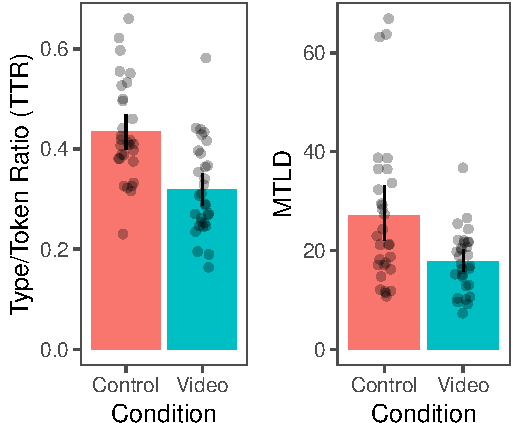
\includegraphics{figs/e1lex_div-1} 

}

\caption[Mean lexical diversity scores by condition (left]{Mean lexical diversity scores by condition (left: Type/Token ratio, right: MTLD) in Experiment 1. Error bars show bootstrapped 95 percent confidence intervals (CIs).}\label{fig:e1lex_div}
\end{figure}
\end{CodeChunk}

Word tokens and word types

\begin{CodeChunk}
\begin{figure}[H]

{\centering 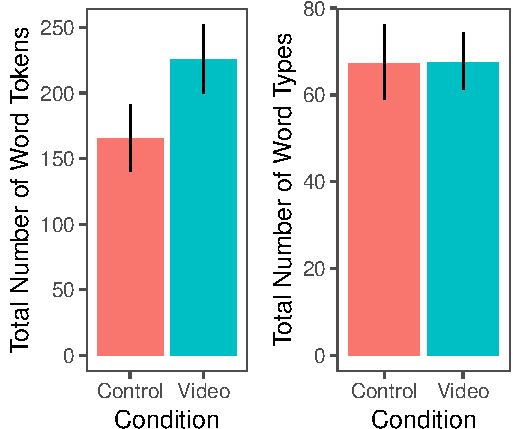
\includegraphics{figs/e1token_type-1} 

}

\caption[Mean number of word types and word tokens by condition in Experiment 1]{Mean number of word types and word tokens by condition in Experiment 1.}\label{fig:e1token_type}
\end{figure}
\end{CodeChunk}

\subsection{Joint Attention}\label{joint-attention}

\begin{CodeChunk}
\begin{figure}[H]

{\centering 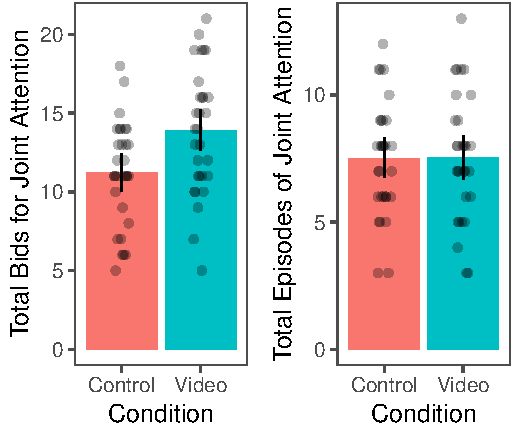
\includegraphics{figs/e1ja-graphs-1} 

}

\caption[Mean number of bids and episodes of Joint Attention in Experiment 1]{Mean number of bids and episodes of Joint Attention in Experiment 1.}\label{fig:e1ja-graphs}
\end{figure}
\end{CodeChunk}

\begin{CodeChunk}
\begin{figure}[H]

{\centering 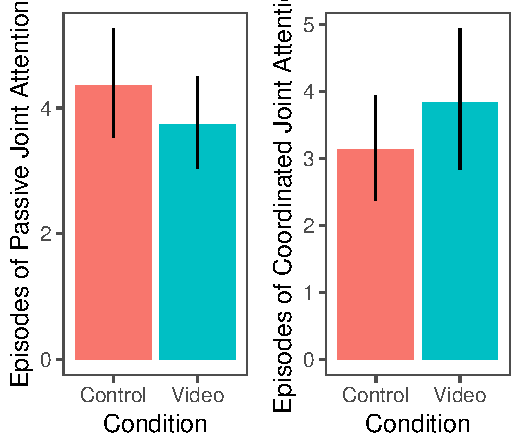
\includegraphics{figs/e1ja-graphs-pass-coord-1} 

}

\caption[Average number of passive and coordinated episodes of JA in Experiment 1]{Average number of passive and coordinated episodes of JA in Experiment 1.}\label{fig:e1ja-graphs-pass-coord}
\end{figure}
\end{CodeChunk}

\subsection{Discussion}\label{discussion}

Both the number of tokens and types are higher in the experimental
condition, while lexical diversity (Type/Token ratio) is higher in the
control condition. Parents may be relatively more repetetive in the
experimental condition since they are attempting to stick to a specific
prescribed task, but they talk more overall. Demographics and PAQ do not
interact with condition, but there is a marginal effect of RR score on
lexical diversity (lower diversity for higher RR scores), and marginal
effects of parent education on word types and tokens (more types and
tokens for higher parent education).

There is (was?) a main effect of condition on total bids for joint
attention. Parents in the experimental condition (i.e., those who saw a
video demonstrating an activity) made a greater number of bids for joint
attention with their child. There was no effect of condition on the
number of episodes of either passive or coordinated joint attention, or
the duration of these episodes. There is a marginal effect of gender on
bids for joint attention, with parents of males producing more bids.
There is a marginal interaction between RR scores and condition on
passive joint attention, such that the experimental condition increased
the number of episodes of PJA to a greater extent for people with high
RR scores. While the electronically-delivered parenting advice increased
the number of bids for joint attention by parents, it did not
significantly effect the number or duration of episodes of joint
attention. One possibility is that child variables had a comparatively
larger impact on the attainment of joint attention.

\section{Experiment 2}\label{experiment-2}

Experiment 1 found that compared to parents who did not watch a video,
parents who watched a Kinedu video spoke more words overall, but had
lower lexical diversity. Parents who watched a video also made more bids
for joint attention, although these bids did not result in more episodes
of joint attention compared to the control group. In Experiment 2 we
attempt to replicate the findings from Experiment 1 with a restricted
number of preregistered predictions. We will additionally include a
second control condition, in which the same activities are described in
written form, rather than being demonstrated in video. This manipulation
will help determine what the contribution of the video demonstration is
in producing the observed effects on parent-child interactions.

\subsection{Method}\label{method-1}

\subsubsection{Participants.}\label{participants.-1}

84 infants (F = 37, M = 47) aged 12-24 months (42 12-17.9 month-olds, 42
18-24 month-olds) and their parents participated in the same museum as
Experiment 1. We included infants who were exposed to English at least
75 percent of the time or who were exposed less but whose participating
parent reported that they primarily speak English with their child at
home. Forty nine\% of participants (n = 41) had been exposed to two or
more languages as indicated by their parent. Parents identified their
children as White (n = 39), Asian (n = 20), African American/Black (n =
1), Biracial (n = 9), other (n = 7), or declined to state (n = 8).
Sixteen parents reported their child was of Hispanic origin. Parents
tended to be highly- educated, with reports of highest level of
education ranging from completed high school (n = 0), some college (n =
5), four-year college (n = 28), some graduate school (n = 2), to
completed graduate school (n = 35) or declined to state (n = 14).

\subsubsection{Materials.}\label{materials.-1}

The design of Experiment 2 was similar to that of Experiment 1, except
that instead of a No-Video control condition, parents instead watched a
video that was generally related to child development research, but did
not give any specific instructions about how to interact with infants or
children. This was to control for the possibility that differences in
language output and joint attention in Experiment 1 could be due to
simply cuing parents to think about infants' learning and cognitive
development. The videos presented in the Control Video condition were
media clips (available on YouTube) of developmental psychologists
explaining their research interleaved with footage of infants or
toddlers engaged in developmental research studies. Thus, the content of
the videos superficially matched those in the Activity Video condition,
but did not suggest any particular activities. The videos were trimmed
to approximately match the average video length in the Activity Video
condition around 1.5 minutes.

\subsubsection{Procedure.}\label{procedure.-1}

The procedure for Experiment 2 matched that of Experiment 1, except that
parents in the Control Video condition watched a control video before
the play session. Consistent with the No-Video control condition in
Experiment 1, parents in the Control Video condition were told to play
with their child as they would at home, and were not given additional
instructions. The coding procedure also matched that of Experiment 1. A
second coder independently coded a third of the videos (i.e., 26 of the
84 videos, approximately equally distributed across ages) to establish
reliability. The two coders had a reliability of ICC = 0.80 with 95\%
confident interval (CI) = {[}0.60,0.90{]} (p \textless{} 0.05) for
number of parent bids for JA; ICC = 0.74 with 95\% CI = {[}0.59,0.87{]}
(p \textless{} 0.05) for number of passive JA episodes; ICC = 0.78 with
95\% CI = {[}0.58,0.90{]} (p \textless{} 0.05) for number of coordinated
JA episodes; ICC = 0.72 with 95\% CI = {[}0.46,0.86{]} (p \textless{}
0.05) for total duration of passive JA episodes, and ICC = 0.88 with
95\% CI = {[}0.75,0.94{]} (p \textless{} 0.05) for total duration of
coordinated JA episodes.

\section{Results}\label{results-1}

Parents' child-directed speech was transcribed and processed in the same
way as in Experiment 1.

\subsection{Lexical Diversity}\label{lexical-diversity-1}

We fit a mixed-effects linear regression predicting TTR and MTLD as a
function of age (scaled and 0-centered) and condition with a random
intercept per video using lme4 (Bates et al., 2015). There was
significantly lower TTR in the Video condition (mean: 0.38) than in the
Control condition (mean: 0.47, \(\beta=-.09\), t(8) = 3.16,
\emph{p}\textless{}.05). There was no significant effect of age. A
similar mixed-effects linear regression instead predicting MTLD found no
significant effects of age or condition. Figure 1 shows the mean of each
lexical diversity measure (TTR and MTLD) by condition.

We also conducted similar regressions predicting the number of word
tokens and types, finding no significant effects of of age or condition.

(Table with mean and SD of tokens, types, and TTR)

\begin{CodeChunk}
\begin{figure}[H]

{\centering 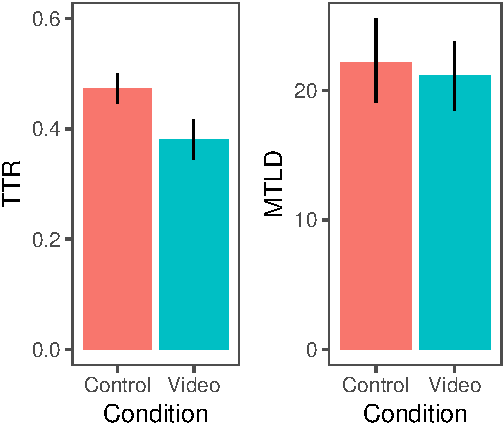
\includegraphics{figs/e2lexdiv-1} 

}

\caption[Mean lexical diversity scores by condition (left]{Mean lexical diversity scores by condition (left: Type/Token ratio, right: MTLD) in Experiment 2.}\label{fig:e2lexdiv}
\end{figure}
\end{CodeChunk}

\begin{CodeChunk}
\begin{figure}[H]

{\centering 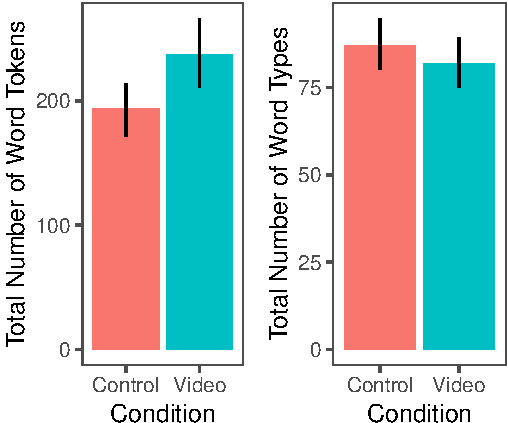
\includegraphics{figs/e2token-type-1} 

}

\caption[Mean number of word types and word tokens by condition in Experiment 2]{Mean number of word types and word tokens by condition in Experiment 2.}\label{fig:e2token-type}
\end{figure}
\end{CodeChunk}

\subsection{Joint Attention}\label{joint-attention-1}

\begin{CodeChunk}
\begin{figure}[H]

{\centering 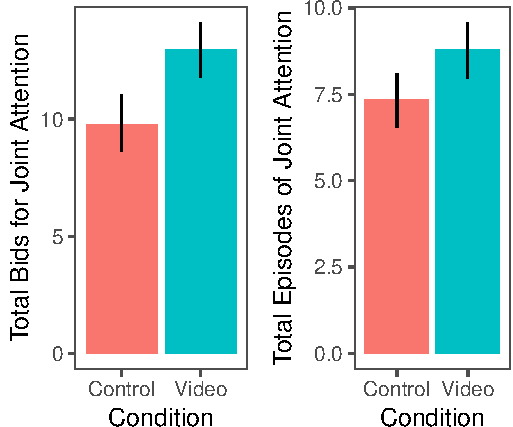
\includegraphics{figs/e2ja-graphs-1} 

}

\caption[Mean number of bids and episodes of Joint Attention in Experiment 2]{Mean number of bids and episodes of Joint Attention in Experiment 2.}\label{fig:e2ja-graphs}
\end{figure}
\end{CodeChunk}

\begin{CodeChunk}
\begin{figure}[H]

{\centering 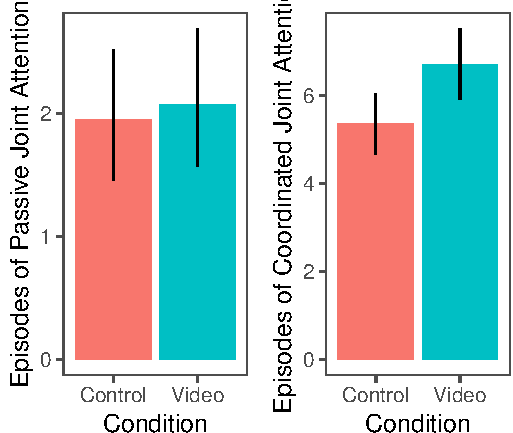
\includegraphics{figs/e2ja-graphs-pass-coord-1} 

}

\caption[Average number of passive and coordinated episodes of JA in Experiment 2]{Average number of passive and coordinated episodes of JA in Experiment 2.}\label{fig:e2ja-graphs-pass-coord}
\end{figure}
\end{CodeChunk}

\section{Discussion}\label{discussion-1}

Similar to results in Experiment 1, the number of tokens was higher in
the experimental condition, while the number of types and lexical
diversity (Type/Token ratio) were higher in the control condition.
Parents may be relatively more repetetive in the experimental condition
since they are attempting to stick to a specific prescribed task, but
they talk more overall. There was a marginal effect of condition on
total bids for joint attention. Parents in the experimental condition
(i.e., those who saw a video demonstrating an activity) made a greater
number of bids for joint attention with their child. There was no effect
of condition on the number of episodes of coordinated joint attention.
There was no effect of condition on the number of episodes of either
passive or coordinated joint attention, or the duration of these
episodes. However, there was a main effect of age on number of episodes
of passive joint attention, duration of passive and coordinated joint
attention, with the older children having fewer episodes of passive
joint attention, shorter duration of passive joint attention, and longer
duration of coordinated joint attention. These results suggest that
children become more socially engaging in interactions with their
caregivers as they develop.

\subsection{Two-column images}\label{two-column-images}

You might want to display a wide figure across both columns. To do this,
you change the \texttt{fig.env} chunk option to \texttt{figure*}. To
align the image in the center of the page, set \texttt{fig.align} option
to \texttt{center}. To format the width of your caption text, you set
the \texttt{num.cols.cap} option to \texttt{2}.

\section{References}\label{references}

\setlength{\parindent}{-0.1in} \setlength{\leftskip}{0.125in} \noindent

\hypertarget{refs}{}
\hypertarget{ref-lme4}{}
Bates, D., Mächler, M., Bolker, B., \& Walker, S. (2015). Fitting linear
mixed-effects models using lme4. \emph{Journal of Statistical Software},
\emph{67}(1), 1--48. \url{http://doi.org/10.18637/jss.v067.i01}

\hypertarget{ref-Bigelow2004}{}
Bigelow, A. E., MacLean, K., \& Proctor, J. (2004). The role of joint
attention in the development of infants' play with objects.
\emph{Developmental Science}, \emph{7}, 518--526.

\hypertarget{ref-Breitenstein2014}{}
Breitenstein, S. M., Gross, D., \& Christophersen, R. (2014). Digital
delivery methods of parenting training interventions: A systematic
review. \emph{Worldviews on Evidence-Based Nursing}, \emph{11},
168--176.

\hypertarget{ref-Hart1995}{}
Hart, B., \& Risley, T. R. (1995). \emph{Meaningful differences in the
everyday experience of young american children}. Baltimore, MD: Brookes.

\hypertarget{ref-Heckman2006}{}
Heckman, J. J. (2006). Skill formation and the economics of investing in
disadvantaged children. \emph{Science}, \emph{312}(5782), 1900--1902.
\url{http://doi.org/10.1126/science.1128898}

\hypertarget{ref-Hirsh2008}{}
Hirsh-Pasek, K., \& Golinkoff, R. M. (2008). Why play= learning.
\emph{Encyclopedia on Early Childhood Development}, 1--7.

\hypertarget{ref-spacy2}{}
Honnibal, I., Matthew AND Montani. (2017). SpaCy 2: Natural language
understanding with bloom embeddings, convolutional neural networks and
incremental parsing. \emph{To Appear}.

\hypertarget{ref-Kaye1970}{}
Kaye, K. (1970). Mother-child instructional interaction.
\emph{Unpublished Doctoral Thesis, Department of Psychology, Harvard
University}.

\hypertarget{ref-Malvern2004}{}
Malvern, D., Richards, B. J., Chipere, N., \& Durán, P. (2004). Lexical
diversity and language development.

\hypertarget{ref-Massey2013}{}
Massey, S. L. (2013). From the reading rug to the play center: Enhancing
vocabulary and comprehensive language skills by connecting storybook
reading and guided play. \emph{Early Childhood Education Journal},
\emph{41}, 125--131.

\hypertarget{ref-McCarthy2010}{}
McCarthy, P. M., \& Jarvis, S. (2010). MTLD, vocd-d, and hd-d: A
validation study of sophisticated approaches to lexical diversity
assessment. \emph{Behavior Research Methods}, \emph{42}(2), 381--392.

\hypertarget{ref-Schulz2007}{}
Schulz, L., \& Bonawitz, E. (2007). Serious fun: Preschoolers engage in
more exploratory play when evidence is confounded. \emph{Developmental
Psychology}, \emph{43}(4), 1045--1050.

\hypertarget{ref-Singer2006}{}
Singer, D. G., Golinkoff, R. M., \& Hirsh-Pasek, K. (Eds.). (2006).
\emph{Play = learning: How play motivates and enhances children's
cognitive and social-emotional growth}. New York, NY: Oxford University
Press.

\hypertarget{ref-Suskind2015}{}
Suskind, D. L., Leffel, K. R., Graf, E., Hernandez, M. W., Gunderson, E.
A., Sapolich, S. G., \ldots{} Levine, S. C. (2015). A parent-directed
language intervention for children of low socioeconomic status: A
randomized controlled pilot study. \emph{Journal of Child Language}.
\url{http://doi.org/10.1017/S0305000915000033}

\hypertarget{ref-datavyu}{}
Team, D. (2014). Datavyu: A video coding tool. \emph{Databrary Project}.
Retrieved from \url{http://datavyu.org}

\hypertarget{ref-Vygotsky1980}{}
Vygotsky, L. S. (1980). Mind in society: The development of higher
psychological processes.

\hypertarget{ref-Weisberg2013}{}
Weisberg, D. S., Hirsh-Pasek, K., \& Golinkoff, R. M. (2013). Guided
play: Where curricular goals meet a playful pedagogy. \emph{Mind, Brain,
and Education}, \emph{7}, 104--112.

\hypertarget{ref-Wood1976}{}
Wood, D., Bruner, J. S., \& Ross, G. (1976). The role of tutoring in
problem solving. \emph{Journal of Child Psychology and Psychiatry},
\emph{17}, 89--100.

\bibliographystyle{apacite}


\end{document}
